% floorplan colorbar: rot — generated, edit freely
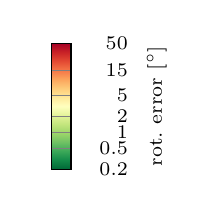
\begin{tikzpicture}[baseline=(current bounding box.north)]
\pgfplotsset{colormap={rdylgnrev}{rgb=(0.0,0.408,0.216) rgb=(0.0729,0.5423,0.286) rgb=(0.2297,0.6581,0.3457) rgb=(0.4359,0.7567,0.392) rgb=(0.6151,0.8353,0.412) rgb=(0.7653,0.9001,0.4897) rgb=(0.8936,0.955,0.6033) rgb=(1.0,1.0,0.749) rgb=(0.9971,0.9129,0.6033) rgb=(0.9943,0.794,0.4743) rgb=(0.987,0.6456,0.3633) rgb=(0.962,0.4634,0.2797) rgb=(0.8919,0.2904,0.2001) rgb=(0.787,0.1343,0.1519) rgb=(0.647,0.0,0.149)}, colormap={rdylgn}{rgb=(0.647,0.0,0.149) rgb=(0.787,0.1343,0.1519) rgb=(0.8919,0.2904,0.2001) rgb=(0.962,0.4634,0.2797) rgb=(0.987,0.6456,0.3633) rgb=(0.9943,0.794,0.4743) rgb=(0.9971,0.9129,0.6033) rgb=(1.0,1.0,0.749) rgb=(0.8936,0.955,0.6033) rgb=(0.7653,0.9001,0.4897) rgb=(0.6151,0.8353,0.412) rgb=(0.4359,0.7567,0.392) rgb=(0.2297,0.6581,0.3457) rgb=(0.0729,0.5423,0.286) rgb=(0.0,0.408,0.216)}}
\begin{axis}[hide axis, scale only axis, width=0pt, height=1.6cm,
  colormap name=rdylgnrev, colorbar, point meta min=-0.699, point meta max=1.699,
  colorbar style={height=1.6cm, width=0.25cm, ylabel={rot.~error [$^\circ$]}, ylabel style={font=\scriptsize},
    ytick={-0.699,-0.301,0.0,0.301,0.699,1.1761,1.699}, yticklabels={0.2,0.5,1,2,5,15,50}, tick label style={font=\scriptsize},
    yticklabel style={text width=1.7em, align=right}}]
  \addplot[draw=none] coordinates {(0,0)};
\end{axis}
\end{tikzpicture}
